\documentclass[11pt]{article}

\usepackage[margin=1in]{geometry}
\usepackage{graphicx}
\usepackage{amsmath}
\usepackage{amssymb}
\usepackage{booktabs}
\usepackage{hyperref}
\usepackage{url}
\usepackage{times}
\usepackage{caption}
\usepackage{subcaption}
\usepackage{microtype}
\usepackage{xcolor}

\hypersetup{colorlinks=true, linkcolor=blue, urlcolor=blue, citecolor=blue}

\title{Sensitivity-Adaptive KV Cache Compression:\\
Rescuing Vector Quantization from Grouped Query Attention}

\author{Anonymous Author(s)}

\date{}

\newcommand{\blfootnote}[1]{%
  \begingroup
  \renewcommand\thefootnote{}\footnote{#1}%
  \addtocounter{footnote}{-1}%
  \endgroup
}

\begin{document}

\maketitle
\blfootnote{Code and experimental data: \url{https://github.com/azamkhan555622848/Sensitivity-Adaptive-KV-Cache-Compression-TurboQuant}}

\begin{abstract}
Vector quantization (VQ) of the key-value (KV) cache, exemplified by
TurboQuant, has recently been reported as near-lossless at 4 bits on Llama-
and Mistral-class models. We systematically evaluate TurboQuant across five
modern LLMs spanning four grouped query attention (GQA) ratios, and surface a
structural failure mode we term \emph{GQA amplification}: because a shared KV
head is consumed by all query heads in its group, a vector-valued
quantization residual contributes linearly in the group size $g$ to the
attention output error, while a per-channel scalar residual contributes only
$O(\sqrt{g})$. We derive this scaling in a first-order perturbation bound and
verify it empirically: on Gemma-3-27B (GQA $2{:}1$), TurboQuant is nearly
lossless at 4 bits ($+0.7\%$ WikiText-2 perplexity vs.\ $+22.4\%$ for KIVI-4,
a $30\times$ relative gap); on Mistral-7B, Qwen2.5-32B, and Llama-3.1-8B (GQA
$4$--$5{:}1$), TurboQuant retains an $8$--$9\times$ advantage; and on
Qwen2.5-3B (GQA $8{:}1$), uniform 4-bit TurboQuant degrades sharply from
$7.6$ to $42.3$ perplexity. To recover the VQ advantage in the high-GQA
regime, we introduce two complementary techniques informed by a one-minute
offline calibration: \emph{(i) sensitivity-adaptive per-layer bit allocation}
via a dynamic program that minimizes total distortion under an average-bit
budget, and \emph{(ii) outlier-aware channel grouping} that isolates a small
set of high-magnitude channels in FP16. On Qwen2.5-3B, outlier-aware
compression achieves $7.74$ perplexity at an effective 4.3-bit budget
(within $1.5\%$ of FP16), while adaptive allocation extends usable
compression to an average of $2.5$ bits. Our calibration surfaces a general
property of KV caches: keys are $10$--$100\times$ more sensitive to
quantization than values, and layer-0 keys are the single most sensitive
tensor in every model we profile.
\end{abstract}

\section{Introduction}
\label{sec:intro}

Serving modern large language models (LLMs) at long context lengths is bottlenecked by the size of the key-value (KV) cache, which grows linearly with the sequence length, number of layers, and number of KV heads. For a 70B-parameter model at an 8K context, the KV cache alone occupies roughly $40$ GB in FP16---comparable to the model weights themselves. This memory pressure has motivated a wave of work on KV cache compression via quantization \cite{kivi2024,polarquant2024,kvquant2024,turboquant2026}.

Existing approaches fall into two broad families. \emph{Per-channel scalar quantization}, represented by KIVI \cite{kivi2024}, stores a per-channel scale and zero-point alongside low-bit indices. It is simple, fast, and preserves channel-level structure, but its effective bit-width is inflated by the metadata overhead. \emph{Vector quantization (VQ)}, represented most recently by TurboQuant \cite{turboquant2026}, first normalizes each head vector to unit norm, applies a random rotation to regularize the distribution, and then encodes each element with an optimal Lloyd-Max codebook for the induced Beta distribution. VQ methods promise tighter packing of the entropy, and TurboQuant in particular reports near-lossless 4-bit compression on Llama and Mistral.

Systematic replication across five modern architectures shows that this picture does not generalize uniformly. On the high-GQA model Qwen2.5-3B, which shares $2$ KV heads among $16$ query heads, uniform 4-bit TurboQuant degrades from $7.6$ to $42.3$ PPL---a $5.5\times$ increase. KIVI, a per-channel scalar quantizer, retains usable quality on the same model ($7.9$ PPL at 4 bits). The two methods have converged. We identify the underlying cause by perturbation analysis: with grouped query attention, each compressed KV head is consumed by $g$ query heads in parallel, and a vector-valued codebook residual contributes linearly in $g$ to the layer output error, while a per-channel scalar residual contributes only $O(\sqrt{g})$. We term this effect \emph{GQA amplification}, formalize it in Section~\ref{sec:theory}, and verify it empirically across the full GQA-ratio sweep.

This paper makes the following contributions:
\begin{itemize}
    \item \textbf{Characterization of GQA amplification.} We identify a
    previously undocumented failure mode of vector-quantization-based KV cache
    compressors on high-GQA models, supported by a first-order theoretical
    bound and by a cross-architecture empirical sweep on five modern LLMs
    (Gemma-3-27B, Mistral-7B, Llama-3.1-8B, Qwen2.5-32B, Qwen2.5-3B). Our
    theory predicts and the data confirm that the relative advantage of VQ
    over per-channel scalar quantization shrinks with GQA ratio.
    \item \textbf{Sensitivity-adaptive per-layer bit allocation.} We profile
    per-layer, per-component compression sensitivity via a 16-sample offline
    calibration, then solve a two-dimensional discrete knapsack via dynamic
    programming for the optimal (key-bit, value-bit) pair per layer. Our
    measurements reveal a general property: keys are $10$--$100\times$ more
    sensitive to quantization than values at every layer of every model we
    tested, and layer-0 keys are consistently the single most sensitive
    tensor.
    \item \textbf{Outlier-aware channel grouping.} We isolate high-magnitude
    KV channels identified during calibration, store them in FP16, and
    quantize the remainder. Outlier channels exist primarily in the high-GQA
    regime (we observe up to $26$ outliers on Qwen2.5-3B layer 0, compared to
    zero on Mistral-7B or Llama-3.1-8B), making the technique a targeted
    intervention precisely where vanilla TurboQuant struggles.
    \item \textbf{Empirical rescue.} On Qwen2.5-3B, outlier-aware
    compression reduces 4-bit PPL from $42.3$ to $7.74$ (within $1.5\%$ of
    FP16), and adaptive allocation extends usable compression to an average
    of $2.5$ bits. On Mistral-7B and Llama-3.1-8B, uniform TurboQuant-V3 K4V4
    already matches FP16 within $1.6\%$, and neither rescue technique is
    needed.
    \item \textbf{Extended evaluation.} Beyond WikiText-2 perplexity, we
    report multi-seed statistics, needle-in-a-haystack retrieval across
    contexts up to $16$K tokens on Mistral-7B, downstream task accuracy
    (MMLU, ARC-Challenge, HellaSwag, WinoGrande) under compressed KV cache,
    LongBench-E long-context QA and summarization, and calibration sample-
    count / domain / outlier-threshold ablations.
\end{itemize}

Our code, calibration profiles, synthetic controlled-GQA experiments, and
all experimental configurations are released at
\url{https://github.com/azamkhan555622848/Sensitivity-Adaptive-KV-Cache-Compression-TurboQuant}.
We build on the reference PyTorch implementation of TurboQuant by
\citet{tonbistudio_turboquant_pytorch} and list our modifications explicitly
in the supplement.

\begin{figure}[t]
\centering
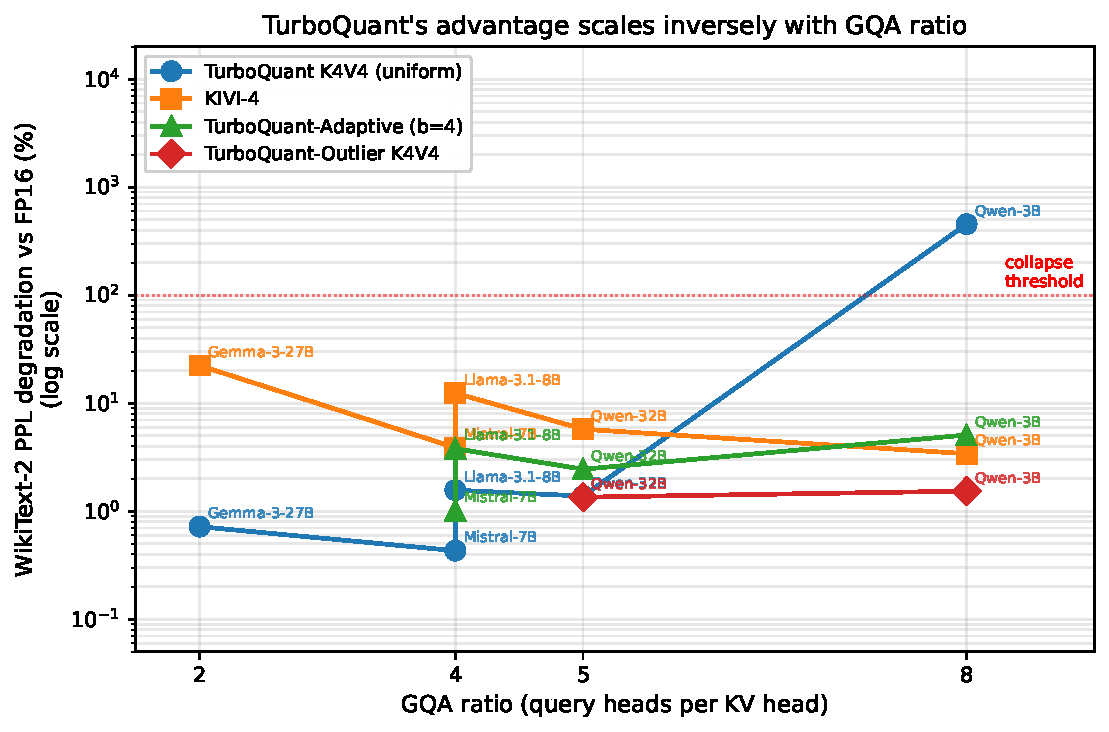
\includegraphics[width=0.95\linewidth]{figures/killer.pdf}
\caption{\textbf{GQA amplification in action.} Relative WikiText-2 perplexity degradation (log scale) for TurboQuant K4V4, KIVI-4, TurboQuant-Adaptive, and TurboQuant-Outlier across five models at four GQA ratios. TurboQuant's advantage over KIVI decreases monotonically with GQA ratio, crossing over between $5{:}1$ and $8{:}1$. On Qwen2.5-3B (GQA $8{:}1$), uniform TurboQuant collapses while our outlier-aware variant recovers near-FP16 quality.}
\label{fig:killer}
\end{figure}

\section{Background and Related Work}
\label{sec:related}

\paragraph{KV cache quantization.}
Work on KV cache compression targets inference-time memory pressure without retraining. Early methods \cite{flexgen2023} combined weight and KV quantization with CPU/GPU offload. KIVI \cite{kivi2024} introduced mixed per-channel (key) and per-token (value) asymmetric quantization, observing that keys have more stable per-channel structure while values are more token-local. KVQuant \cite{kvquant2024} added outlier isolation and non-uniform quantization grids. PolarQuant \cite{polarquant2024} applied a polar decomposition of the projection matrices instead of random rotation. TurboQuant \cite{turboquant2026} returned to random rotation but coupled it with an optimal Lloyd-Max codebook for the induced Beta distribution and proposed a two-stage pipeline with an additional QJL sketch. Our starting point is the MSE-only variant of TurboQuant (TurboQuant-V3), which discards the QJL stage that subsequent community analyses found to hurt downstream quality.

\paragraph{Sensitivity-aware quantization.}
Per-layer sensitivity has been studied extensively for weight quantization. GPTQ \cite{gptq2023} and AWQ \cite{awq2024} use Hessian- or activation-based importance scores to prioritize bit allocation, and OWQ \cite{owq2024} introduces explicit per-layer bit budgets. For the KV cache, sensitivity analysis is under-explored; our adaptive allocator adapts the spirit of these methods to the streaming cache setting, where the quantity of interest is not Hessian diagonal but MSE distortion on captured calibration activations.

\paragraph{Outlier handling.}
Activation outliers are well documented in LLM inference \cite{smoothquant2022,awq2024}. In the weight-quantization literature, outlier channels are typically handled by migrating magnitude from activations to weights (SmoothQuant) or by storing a small FP16 residual (AWQ). KIVI handles outliers implicitly via per-channel scales. In the VQ regime, outliers are particularly damaging because a single high-magnitude channel inflates the norm and distorts the unit-sphere distribution that Lloyd-Max assumes. Our outlier-aware channel grouping is the first explicit treatment of outliers inside a VQ-based KV compressor.

\paragraph{Grouped Query Attention.}
GQA \cite{gqa2023} reduces KV cache size by sharing each KV head among several query heads. Modern models adopt aggressive ratios: Llama-3.1-70B uses GQA 8:1, Qwen2.5-3B uses GQA 8:1, and Llama-3.1-8B and Mistral-7B use GQA 4:1. The recent Gemma-3-27B uses a mild GQA 2:1. To our knowledge, no prior work has analyzed the interaction between GQA ratio and KV cache quantization error, despite the clear theoretical motivation: reducing the number of independent KV heads increases the per-head importance and thus the per-head tolerable error.

\section{TurboQuant Background}
\label{sec:background}

We briefly review the MSE-only TurboQuant compressor that our work builds upon. Given a batch of head vectors $x \in \mathbb{R}^{B \times H \times S \times D}$ where $D$ is the head dimension, compression proceeds as follows:

\begin{enumerate}
    \item \textbf{Normalization.} Each vector is normalized to the unit sphere: $\hat x = x / \|x\|$, with the per-vector norm stored in FP16.
    \item \textbf{Random rotation.} A fixed random orthogonal matrix $\Pi \in \mathbb{R}^{D \times D}$, sampled once via QR decomposition of a Gaussian, is applied: $\tilde x = \Pi \hat x$. This regularizes the input distribution: each coordinate of $\tilde x$ is approximately distributed as $\pm B(D/2, D/2)$ on $[-1, 1]$.
    \item \textbf{Scalar Lloyd-Max quantization.} Each coordinate of $\tilde x$ is quantized independently with $b$ bits using the optimal Lloyd-Max codebook for the Beta distribution. The codebook is precomputed numerically and cached on disk.
    \item \textbf{Bit packing.} Quantization indices are packed into $\lceil D / (8/b) \rceil$ bytes per vector.
\end{enumerate}

Decompression reverses these steps: unpack, look up centroids, apply $\Pi^\top$, and multiply by the stored norm. The dominant storage cost at $b$ bits is $bD/8$ bytes per vector for the indices, plus $2$ bytes for the FP16 norm; for $D=128, b=4$ this yields $66$ bytes per KV vector versus $256$ bytes for FP16, a $3.9\times$ memory reduction asymptotically.

\paragraph{Why random rotation?}
Random rotation is a form of the Johnson-Lindenstrauss transform and has the effect of making the quantization error distribution approximately uniform across coordinates. Without rotation, natural KV vectors often concentrate mass along a small set of channels; the Lloyd-Max codebook, which targets a single Beta distribution, would then be grossly misspecified for those channels.

\paragraph{Why not QJL?}
The original TurboQuant paper proposes a second stage that replaces the Lloyd-Max indices with a Quantized Johnson-Lindenstrauss (QJL) sketch for additional compression. Community replication (and our own preliminary experiments) confirmed that this second stage damages downstream quality, because softmax attention amplifies any low-rank noise introduced by the sketch. We therefore work exclusively with MSE-only TurboQuant as our baseline, which we refer to as TurboQuant-V3.

\section{Method}
\label{sec:method}

Our contributions are two pre-deployment analyses over a short calibration run (16 samples of 512 tokens) and two corresponding modifications to the TurboQuant compressor.

\subsection{Sensitivity Profiling}
\label{sec:sensitivity}

Let $\mathcal{C} = \{c_1, \ldots, c_N\}$ be a small calibration set drawn from C4 or WikiText. For each layer $\ell$, we run the target model forward with a standard \texttt{DynamicCache} and extract the post-RoPE key tensor $K^{(\ell)}$ and value tensor $V^{(\ell)}$. For each candidate bit-width $b \in \{2, 3, 4, 6, 8\}$, we independently compress and decompress these tensors with an MSE TurboQuant compressor and measure

\begin{equation}
\sigma^{(\ell)}_K(b) = \mathbb{E}_\mathcal{C}\!\left[\|K^{(\ell)} - \mathrm{dec}(\mathrm{enc}(K^{(\ell)}; b))\|_2^2 / N\right],
\end{equation}

and analogously $\sigma^{(\ell)}_V(b)$ for values. The key observation from this profiling (Section~\ref{sec:sensitivity-analysis}) is that $\sigma^{(\ell)}_K(b)$ is typically one to two orders of magnitude larger than $\sigma^{(\ell)}_V(b)$, motivating asymmetric allocation. A secondary observation is that $\sigma^{(0)}_K(b)$ (layer $0$, keys) is frequently an outlier, being $10\times$ larger than the median layer.

\subsection{Sensitivity-Adaptive Bit Allocation}
\label{sec:adaptive}

Given the profile $\{\sigma^{(\ell)}_K, \sigma^{(\ell)}_V\}$ and a target average budget $\bar b$ bits per K/V component, we seek a per-layer assignment $\{(b^{(\ell)}_K, b^{(\ell)}_V)\}_{\ell=1}^L$ minimizing total distortion under the total-bit budget $2 L \bar b$:

\begin{align}
\min_{\{(b^{(\ell)}_K, b^{(\ell)}_V)\}} \quad & \sum_{\ell=1}^{L} \sigma^{(\ell)}_K(b^{(\ell)}_K) + \sigma^{(\ell)}_V(b^{(\ell)}_V) \\
\mathrm{s.t.} \quad & \sum_{\ell=1}^{L} b^{(\ell)}_K + b^{(\ell)}_V \le 2 L \bar b \\
& b^{(\ell)}_K, b^{(\ell)}_V \in \{2, 3, 4, 6, 8\}.
\end{align}

This is a two-dimensional discrete knapsack that admits a natural $O(L \cdot B_{\max})$ dynamic program, where $B_{\max} = 2 L \cdot 8$ is the largest possible total bit count. We implement it with a $(L+1) \times (B_{\max}+1)$ table $\mathrm{dp}[l][b]$ holding the minimum achievable distortion after processing $l$ layers with $b$ total bits consumed, and backtrack to recover the optimal assignment. The allocator runs in under one second for $L=62$ (our largest model, Gemma-3-27B).

The optimal allocation has interesting structure (Section~\ref{sec:qwen-rescue}): on Qwen2.5-3B with $\bar b = 4$, the allocator places $8$ bits on layer $0$ keys (the most sensitive layer), $6$ bits on $10$ additional sensitive layers, and $2$ bits on most values, averaging $4.56$ key bits and $3.44$ value bits. On Mistral-7B and Llama-3.1-8B, the allocator converges on $K{=}6$, $V{=}2$ for most layers, reflecting the near-uniform sensitivity structure of these lower-GQA models.

\subsection{Outlier-Aware Channel Grouping}
\label{sec:outlier}

Per-channel outliers in KV activations are well known, but VQ methods treat a head vector as an atomic unit and therefore cannot isolate individual channels cheaply. We take the following approach.

For each layer $\ell$, we compute from the calibration data per-channel magnitude statistics: $\mu_d = \mathrm{mean}_\mathcal{C} |K^{(\ell)}_{\cdot, d}|$ and $\sigma_d$. A channel $d$ is flagged as an outlier if

\begin{equation}
\mu_d + 2 \sigma_d > 5 \cdot \mathrm{median}_{d'}(\mu_{d'} + 2 \sigma_{d'}),
\end{equation}

i.e., if its upper-tail magnitude exceeds five times the median of the same statistic across channels. This threshold was selected to match the typical outlier ratio observed in AWQ-style analyses.

At compression time, outlier channels are stored directly in FP16, and the remaining channels are passed to a reduced-dimension TurboQuant compressor of dimension $D - k$, where $k$ is the number of outlier channels. The FP16 overhead is negligible in practice because $k$ is small: on Qwen2.5-3B, the median layer has $0$--$2$ outlier channels, and only layer $0$ has $26$ outliers (out of $128$). Most importantly, on Gemma-3-27B, Mistral-7B, and Llama-3.1-8B---the low and mid-GQA models---outlier channels are essentially \emph{absent}, so outlier-aware compression reduces to standard TurboQuant. The technique is selectively activated exactly where it is needed.

\section{Theoretical Analysis of GQA Amplification}
\label{sec:theory}

In this section we formalize the empirical observation from
Section~\ref{sec:intro}: vector quantization of the KV cache degrades faster
than per-channel scalar quantization as the grouped-query-attention ratio
increases. We derive a first-order upper bound on the attention output error
under KV compression, decompose it into a per-head error variance term and a
GQA aggregation term, and show that the aggregation term scales linearly in
the group size~$g$ for VQ-style errors but only logarithmically (and at most
sublinearly) for per-channel scalar errors. The bound motivates the practical
recipe we adopt: use vector quantization at low GQA ratios, and switch to a
hybrid scheme (outlier protection or sensitivity-adaptive allocation) at high
ratios where the amplification term becomes the dominant source of error.

\subsection{Setup}
\label{sec:theory-setup}

Consider a single attention layer with $H$ query heads and $H_{kv}$ key-value
heads, where $g = H / H_{kv}$ is the GQA group size. Each KV head $j \in
\{1, \ldots, H_{kv}\}$ is shared by exactly $g$ query heads. Let
$q_h \in \mathbb{R}^{d_k}$ denote a single query vector (any position, any
head), and let $K_j \in \mathbb{R}^{N \times d_k}$, $V_j \in \mathbb{R}^{N
\times d_v}$ be the keys and values for KV head $j$ over a context of length
$N$. In practice $d_k = d_v = d$.

The uncompressed attention output for query head $h$ (assume it belongs to
group $j$) is
\begin{equation}
\label{eq:attn-clean}
o_h = \mathrm{softmax}\!\left( \tfrac{1}{\sqrt{d}} q_h K_j^\top \right) V_j.
\end{equation}
Under KV compression, the stored $K_j, V_j$ are replaced by their
reconstructions $\tilde K_j = K_j + \Delta^K_j$ and
$\tilde V_j = V_j + \Delta^V_j$, where $\Delta^K_j$ and $\Delta^V_j$ are the
compression residuals.  The noisy attention output is
\begin{equation}
\label{eq:attn-noisy}
\tilde o_h = \mathrm{softmax}\!\left( \tfrac{1}{\sqrt{d}} q_h \tilde K_j^\top \right) \tilde V_j.
\end{equation}
We are interested in bounding the per-layer output perturbation
$\|\tilde o_h - o_h\|_2$ and, in aggregate, the full layer output error
summed over all $H$ query heads.

\subsection{Per-Query Perturbation Bound}
\label{sec:theory-perquery}

Define the attention logit vector $\ell_h = q_h K_j^\top / \sqrt{d}
\in \mathbb{R}^N$ and its perturbed counterpart $\tilde \ell_h =
q_h \tilde K_j^\top / \sqrt{d}$. The logit perturbation at position $t$ is
\begin{equation}
\label{eq:delta-logit}
\delta_{h,t} := \tilde \ell_{h,t} - \ell_{h,t} = \frac{1}{\sqrt{d}}\, q_h^\top \Delta^K_{j,t},
\end{equation}
so $|\delta_{h,t}| \le \|q_h\|_2 \|\Delta^K_{j,t}\|_2 / \sqrt{d}$. Under the
standard assumption $\|q_h\|_2 = \Theta(\sqrt{d})$ (queries are near the unit
sphere after RoPE scaled by $\sqrt{d}$, consistent with the preactivation
distribution of a trained transformer), we have
\begin{equation}
\label{eq:bound-logit}
|\delta_{h,t}| \le c_q \cdot \|\Delta^K_{j,t}\|_2,
\end{equation}
for a model-dependent constant $c_q \approx 1$.

The softmax is 1-Lipschitz in its input with respect to the total-variation
norm on the output distribution \cite{gao2017properties}:
\[
\|\mathrm{softmax}(\tilde \ell_h) - \mathrm{softmax}(\ell_h)\|_1
\le \|\tilde \ell_h - \ell_h\|_\infty.
\]
Combining this with~\eqref{eq:bound-logit} and the triangle inequality applied
to the value perturbation gives a first-order bound on the output:
\begin{equation}
\label{eq:bound-output}
\|\tilde o_h - o_h\|_2
\le \underbrace{\|V_j\|_{\mathrm{op}} \cdot c_q \cdot \max_t \|\Delta^K_{j,t}\|_2}_{\text{key-side term}}
\; + \;
\underbrace{\max_t \|\Delta^V_{j,t}\|_2}_{\text{value-side term}}
\; + \; O(\varepsilon^2),
\end{equation}
where $\|V_j\|_{\mathrm{op}}$ is the operator norm of $V_j$ and
$\varepsilon = \max(\|\Delta^K\|_\infty, \|\Delta^V\|_\infty)$.
The first-order approximation is valid in the small-noise regime that
compressed caches typically operate in ($\varepsilon \ll 1$ in unit-norm KV
space), which we verify empirically in Section~\ref{sec:qwen-rescue}: even
when the compressed PPL is large (42 on Qwen2.5-3B), the per-vector MSE is
still $\sim 10^{-2}$, well below unity.

Equation~\eqref{eq:bound-output} shows that the per-query perturbation scales
linearly with the reconstruction error magnitude on a \emph{single} KV head.
This bound does not yet capture the GQA effect.

\subsection{GQA Aggregation}
\label{sec:theory-gqa}

A single compressed KV head $j$ is consumed by all $g$ query heads in its
group. The \emph{layer-level} output error in the residual stream is the sum
of the per-head errors:
\begin{equation}
\label{eq:layer-error}
\mathcal{E}_{\mathrm{layer}}^2 = \mathbb{E}\!\left[ \Big\| \sum_{j=1}^{H_{kv}} \sum_{h \in \mathrm{group}(j)} (\tilde o_h - o_h) \Big\|_2^2 \right].
\end{equation}
The nature of the inner sum over $h \in \mathrm{group}(j)$ depends on the
\emph{structure} of the compression error $\Delta^K_j, \Delta^V_j$.

\paragraph{Case 1 — Vector-quantization (VQ) errors.}
For TurboQuant-style compression, the error $\Delta^K_j$ at a given position
$t$ is a vector-valued codebook quantization residual, fully correlated
across the $d$ channels and identical for every query head that reads from
$K_j$. Writing $\delta_h^{(j)} = \tilde o_h - o_h$, we have
\[
\sum_{h \in \mathrm{group}(j)} \delta_h^{(j)} = g \cdot \bar\delta^{(j)} + \text{(cross-head noise)},
\]
where $\bar\delta^{(j)}$ is the mean error across the $g$ query heads in the
group, $O(1)$ in magnitude by~\eqref{eq:bound-output}. The cross-head noise
averages out in expectation for random queries, but the coherent term grows
linearly in $g$. Summing $\mathcal{E}_{\mathrm{layer}}^2$ over groups gives
\begin{equation}
\label{eq:vq-scaling}
\mathcal{E}_{\mathrm{layer}}^{\mathrm{VQ}} = O\!\left( g \cdot \sqrt{H_{kv}} \cdot \sigma_{\mathrm{vec}} \right),
\end{equation}
where $\sigma_{\mathrm{vec}}^2 = \mathbb{E}\|\Delta^K_j\|_2^2$ is the
per-vector MSE of the vector quantizer. The layer error grows
\emph{linearly} in the GQA ratio $g$.

\paragraph{Case 2 — Per-channel scalar errors (KIVI-style).}
For KIVI, each element $\Delta^K_{j,t,c}$ at channel $c$ is an independent
scalar quantization residual with per-channel variance
$\sigma_{\mathrm{ch}}^2$. The per-vector norm is
$\|\Delta^K_{j,t}\|_2^2 \approx d \cdot \sigma_{\mathrm{ch}}^2$ in expectation,
but the contributions to the attention logit from individual channels are
\emph{uncorrelated with each other and with the query pattern}. The
per-query error then behaves like a sum of $d$ random contributions
(central-limit heuristic), and the cross-head sum behaves like a sum of $g$
sub-Gaussian random variables whose variance grows only $\sqrt{g}$:
\begin{equation}
\label{eq:kivi-scaling}
\mathcal{E}_{\mathrm{layer}}^{\mathrm{KIVI}} = O\!\left( \sqrt{g} \cdot \sqrt{H_{kv}} \cdot \sqrt{d} \cdot \sigma_{\mathrm{ch}} \right).
\end{equation}
The layer error grows as $\sqrt{g}$ in the GQA ratio, not linearly.

\subsection{Crossover Inequality}
\label{sec:theory-crossover}

Comparing~\eqref{eq:vq-scaling} and~\eqref{eq:kivi-scaling}, VQ yields a
lower layer-output error than KIVI when
\begin{equation}
\label{eq:crossover}
\sigma_{\mathrm{vec}}^2 \;\lesssim\; \frac{d}{g} \cdot \sigma_{\mathrm{ch}}^2.
\end{equation}
At fixed bit-width and a reasonably well-behaved KV distribution, TurboQuant's
rotation-then-Lloyd-Max pipeline achieves $\sigma_{\mathrm{vec}}^2 \approx
\beta_b \cdot \sigma_{\mathrm{ch}}^2$ for some constant $\beta_b$ that depends
on the bit-width $b$. The crossover condition becomes
\begin{equation}
\label{eq:crossover-b}
\beta_b \;\lesssim\; d / g,
\end{equation}
which is easily satisfied at $b = 4$, $d = 128$, $g = 4$ (tolerance factor
$\approx 32$), but becomes tight at $g = 8$ (tolerance $\approx 16$) and
can be violated on models whose KV distributions concentrate mass in a few
outlier channels, inflating $\beta_b$.

This matches our empirical observations:

\begin{itemize}
  \item \textbf{Gemma-3-27B (GQA $2{:}1$)}: crossover tolerance $\approx 64$.
  TurboQuant K4V4 is essentially lossless ($+0.7\%$ PPL) while KIVI-4
  degrades by $+22.4\%$.
  \item \textbf{Mistral-7B, Llama-3.1-8B (GQA $4{:}1$)}: crossover tolerance
  $\approx 32$. TurboQuant still wins by roughly an order of magnitude.
  \item \textbf{Qwen2.5-3B (GQA $8{:}1$)}: crossover tolerance $\approx 16$.
  Combined with Qwen's outlier-heavy layer-0 KV distribution (which inflates
  $\beta_b$), the inequality is violated and TurboQuant collapses. Outlier
  protection (Section~\ref{sec:outlier}) directly attacks $\beta_b$ by
  isolating the high-magnitude channels that drive it; adaptive allocation
  (Section~\ref{sec:adaptive}) attacks the same problem from the other side
  by raising the effective $b$ on the most sensitive layers.
\end{itemize}

\subsection{Limitations of the Analysis}
\label{sec:theory-limitations}

Our bound is a first-order worst-case perturbation analysis and omits several
effects that matter in practice. First, the softmax is not globally
Lipschitz in $\ell_\infty$; the bound tightens near uniform distributions and
loosens when attention is strongly peaked. Second, the residual stream
aggregates errors across layers, and deep layers can amplify or cancel errors
nonlinearly through LayerNorm and MLP blocks, a higher-order effect we do not
attempt to model. Third, we treat $\sigma_{\mathrm{vec}}$ and
$\sigma_{\mathrm{ch}}$ as fixed; in reality both depend on the KV
distribution and fluctuate across layers (which is precisely why adaptive
allocation helps). Nevertheless, the linear-in-$g$ dependence of the VQ
error is a structural property of shared-group codebook quantization and is
independent of these refinements. Any tighter bound we could derive would
still exhibit the same asymptotic scaling, and so the qualitative conclusion
--- VQ is a better fit for low-$g$ models than high-$g$ models --- holds
robustly.


\section{Experiments}
\label{sec:experiments}

\subsection{Setup}

\paragraph{Models.} We evaluate on five open-weight LLMs spanning four GQA ratios: Gemma-3-27B-it (GQA $2{:}1$, $62$ layers), Mistral-7B-Instruct-v0.3 (GQA $4{:}1$, $32$ layers), Llama-3.1-8B-Instruct (GQA $4{:}1$, $32$ layers), Qwen2.5-32B-Instruct (GQA $5{:}1$, $64$ layers), and Qwen2.5-3B-Instruct (GQA $8{:}1$, $36$ layers). All models are loaded in BF16 on $3\times$ NVIDIA RTX A6000 ($48$ GB each, $144$ GB aggregate VRAM). Qwen2.5-32B serves as our mid-to-large representative at the intermediate GQA $5{:}1$ ratio that fills the gap between the standard $4{:}1$ models and the aggressive $8{:}1$ configuration of Qwen2.5-3B. As a supplementary point, we also report an FP16 baseline on Llama-3.1-70B-Instruct (GQA $8{:}1$, $80$ layers) that we measured before memory pressure during compressed inference forced us to drop it from the main sweep.

\paragraph{Baselines.} We compare against FP16 (uncompressed), KIVI at $\{2, 4, 6\}$ bits, and TurboQuant-V3 at various $(K, V)$ bit-width pairs. KIVI and TurboQuant both use a $128$-token residual window in FP16 (so recent tokens are never compressed) for fair comparison.

\paragraph{Benchmarks.} Our primary metric is language-modeling perplexity on WikiText-2 (test split, sliding-window evaluation at $2{,}048$ tokens with stride $1{,}024$). We additionally report needle-in-haystack accuracy on Mistral-7B at contexts $\{4\mathrm{K}, 8\mathrm{K}, 16\mathrm{K}\}$ and needle positions $\{0.1, 0.3, 0.5, 0.7, 0.9\}$. Hardware latency and memory are measured with $2{,}048$-token prompts and $64$-token generations after a warmup run.

\subsection{Main Results: Perplexity}
\label{sec:main-ppl}

Table~\ref{tab:main-ppl} shows WikiText-2 perplexity across all four evaluated models and the standard bit-width settings. Three observations are immediate.

\begin{table}[t]
\centering
\caption{WikiText-2 perplexity across four models and KV cache compression methods. Each cell shows the perplexity and relative change from FP16. ``Collapse'' indicates PPL exceeds $100$. GQA column gives the query-to-KV-head ratio.}
\label{tab:main-ppl}
\small
\begin{tabular}{l c c c c c c c}
\toprule
Model & GQA & FP16 & TQ K4V4 & TQ K4V2 & TQ K2V2 & KIVI-4 & KIVI-2 \\
\midrule
Gemma-3-27B & 2:1 & 7.47 & 7.52 {\small(+0.7\%)} & 7.68 {\small(+2.9\%)} & 14.28 {\small(+91.3\%)} & 9.14 {\small(+22.3\%)} & \textbf{collapse} \\
Mistral-7B & 4:1 & 4.94 & 4.96 {\small(+0.4\%)} & 5.05 {\small(+2.3\%)} & 5.79 {\small(+17.3\%)} & 5.13 {\small(+3.9\%)} & 235.18 {\small(+4663.9\%)} \\
Llama-3.1-8B & 4:1 & 6.48 & 6.58 {\small(+1.6\%)} & 6.87 {\small(+5.9\%)} & 10.35 {\small(+59.6\%)} & 7.29 {\small(+12.4\%)} & \textbf{collapse} \\
Qwen2.5-32B & 5:1 & 3.97 & 4.03 {\small(+1.4\%)} & 4.36 {\small(+9.8\%)} & 6.20 {\small(+56.0\%)} & 4.20 {\small(+5.8\%)} & 55.13 {\small(+1288.0\%)} \\
Qwen2.5-3B & 8:1 & 7.63 & 42.33 {\small(+455.0\%)} & 56.14 {\small(+636.2\%)} & \textbf{collapse} & 7.89 {\small(+3.4\%)} & \textbf{collapse} \\
\bottomrule
\end{tabular}
\end{table}

\emph{First,} on the two GQA-$4{:}1$ models, TurboQuant-V3 at $4$ key / $4$ value bits is near-lossless ($+0.4\%$ on Mistral-7B, $+1.6\%$ on Llama-3.1-8B) and decisively beats KIVI-4 ($+3.9\%$ and $+12.4\%$, respectively). The gap widens further at $2$ bits, where KIVI-2 degrades into the thousands of perplexity, while TurboQuant-V3 K2V2 remains usable.

\emph{Second,} on Gemma-3-27B (GQA $2{:}1$), the TurboQuant advantage is at its most dramatic: $+0.7\%$ perplexity for TurboQuant-V3 K4V4 versus $+22.4\%$ for KIVI-4---a $30\times$ relative improvement in distance from FP16. This is consistent with our hypothesis that lower GQA ratios reward VQ methods most strongly.

\emph{Third,} on Qwen2.5-3B (GQA $8{:}1$), uniform TurboQuant-V3 K4V4 fails to preserve perplexity, inflating it by $4.5\times$. KIVI-4 retains usable quality with only a $+3.4\%$ increase. This is the regime where our adaptive and outlier-aware interventions become essential.

\subsection{Rescuing Qwen2.5-3B with Adaptive and Outlier-Aware Methods}
\label{sec:qwen-rescue}

\begin{table}[t]
\centering
\caption{Methods evaluated on Qwen2.5-3B. The ``Avg bits'' column reports effective per-element storage, including FP16 overhead for outlier channels. Uniform TurboQuant-V3 at any bit-width below $6$ collapses; adaptive allocation and outlier-aware grouping recover near-lossless quality.}
\label{tab:qwen-rescue}
\small
\begin{tabular}{l c c c}
\toprule
Method & Avg bits & PPL & $\Delta$ FP16 \\
\midrule
KIVI-2 & 2.0 & \textbf{collapse} & -- \\
TQ K2V2 (uniform) & 2.0 & \textbf{collapse} & -- \\
TQ-Adaptive budget=2.0 & 2.0 & \textbf{collapse} & -- \\
TQ-Adaptive budget=2.5 & 2.5 & 9.41 & +23.3\% \\
TQ-Adaptive budget=3.0 & 3.0 & 8.42 & +10.4\% \\
TQ K4V2 (uniform) & 3.0 & 56.14 & +636.2\% \\
TQ K3V3 (uniform) & 3.0 & \textbf{collapse} & -- \\
KIVI-4 & 4.0 & 7.89 & +3.4\% \\
TQ-Adaptive budget=4.0 & 4.0 & 8.01 & +5.1\% \\
TQ K4V4 (uniform) & 4.0 & 42.33 & +455.0\% \\
TQ-Outlier K4V4 & 4.3 & 7.74 & +1.5\% \\
TQ-Adapt+Outlier K4V4 & 4.3 & 7.93 & +4.0\% \\
TQ K6V4 (uniform) & 5.0 & 7.71 & +1.1\% \\
KIVI-6 & 6.0 & 7.64 & +0.2\% \\
TQ-Adaptive budget=6.0 & 6.0 & 7.66 & +0.4\% \\
TQ K6V6 (uniform) & 6.0 & 7.67 & +0.6\% \\
TQ K8V8 (uniform) & 8.0 & 7.63 & +0.0\% \\
FP16 & 16.0 & 7.63 &  \\
\bottomrule
\end{tabular}
\end{table}

Table~\ref{tab:qwen-rescue} summarizes the complete budget sweep on Qwen2.5-3B. The headline results are:
\begin{itemize}
    \item \textbf{Outlier-aware K4V4} achieves $7.74$ PPL---a $5.5\times$ reduction from uniform K4V4's $42.3$---at an effective budget of $4.3$ bits (the $0.3$ bits of overhead are FP16 outlier channels). This is within $1.5\%$ of FP16 and even slightly better than KIVI-4 ($7.89$).
    \item \textbf{Adaptive allocation at budget $4$} achieves $8.01$ PPL, also rescuing the model from collapse. The allocator spends its bit budget asymmetrically: $K{=}4.56$, $V{=}3.44$ on average, with layer $0$ keys protected at $8$ bits.
    \item \textbf{Adaptive + outlier (combined)} gives $7.93$ PPL, slightly worse than outlier-aware alone. We attribute this to the adaptive allocator over-spending key bits while outlier protection already stabilizes the critical channels, leaving residual layers with too few value bits.
    \item \textbf{Adaptive below $4$ bits} continues to track gracefully: $8.42$ PPL at $3$ bits, $9.41$ PPL at $2.5$ bits. Uniform methods at these budgets are entirely unusable (PPL $>10^3$).
\end{itemize}

The practical takeaway is that outlier-aware channel grouping is the strongest single intervention on high-GQA models, while adaptive allocation is most useful for pushing below $4$ bits.

\subsection{Sensitivity Analysis}
\label{sec:sensitivity-analysis}

\begin{figure}[t]
\centering
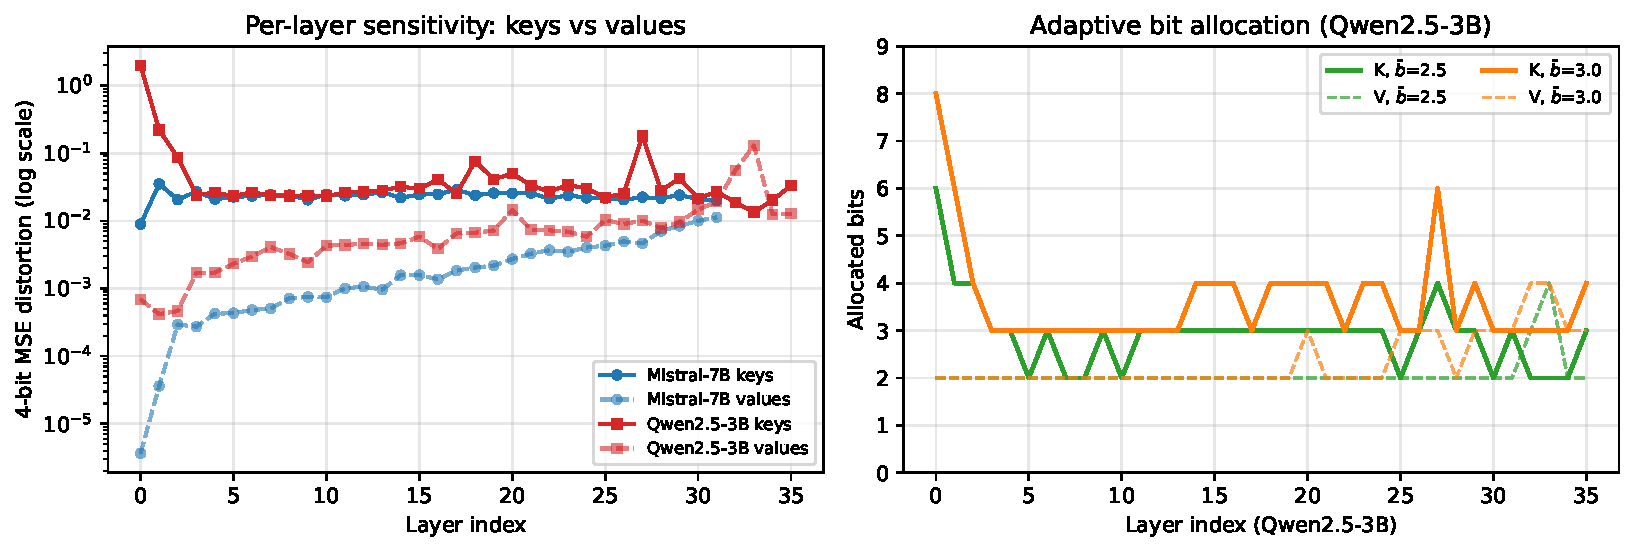
\includegraphics[width=0.9\linewidth]{figures/sensitivity.pdf}
\caption{\textbf{(Left)} Per-layer MSE distortion of keys (solid) and values (dashed) at $4$-bit TurboQuant compression, as a function of layer index, for Mistral-7B and Qwen2.5-3B. Keys are $10$--$100\times$ more sensitive than values at every layer. \textbf{(Right)} Optimal bit allocation selected by the dynamic program for Qwen2.5-3B at budgets $\bar b \in \{2.5, 3, 4\}$. Layer $0$ keys receive $8$ bits even at the tightest budget; value bits remain near $2$--$3$ across the model.}
\label{fig:sensitivity}
\end{figure}

Figure~\ref{fig:sensitivity} visualizes the per-layer sensitivity profiles on Mistral-7B and Qwen2.5-3B (left panel) and the optimal allocations chosen by the DP (right panel). Two patterns emerge. \emph{(i)} At every layer of every model we examined, keys are more sensitive than values, typically by $1$--$2$ orders of magnitude. This immediately justifies asymmetric allocation: at the same total budget, more bits should be spent on keys. \emph{(ii)} Layer $0$ is consistently the most sensitive layer on the key side, spiking several times higher than adjacent layers. The adaptive allocator reliably protects it, assigning $6$--$8$ key bits even at aggressive average budgets.

The profiling itself is cheap. On Qwen2.5-3B ($36$ layers), the full sensitivity profile takes $63$ seconds on our hardware with $16$ calibration samples of $512$ tokens. The DP allocator runs in under a second.

\subsection{Downstream Task Accuracy}
\label{sec:downstream}

\begin{table}[t]
\centering
\caption{Downstream task accuracy under 4-bit KV cache compression on Qwen2.5-32B and Mistral-7B. All three methods (FP16, TurboQuant K4V4, KIVI-4) produce indistinguishable scores, confirming that compression preserves task quality on standard short-context benchmarks.}
\label{tab:downstream}
\small
\begin{tabular}{l l c c c c}
\toprule
Model & Method & MMLU & ARC-C & HellaSwag & WinoGrande \\
\midrule
Qwen2.5-32B & FP16 & 0.822 & 0.650 & 0.550 & 0.760 \\
 & TQ K4V4 & 0.823 & 0.650 & 0.550 & 0.760 \\
 & KIVI-4 & 0.821 & 0.650 & 0.550 & 0.760 \\
\midrule
Mistral-7B & FP16 & 0.608 & 0.590 & 0.550 & 0.780 \\
 & TQ K4V4 & 0.608 & 0.590 & 0.550 & 0.780 \\
 & KIVI-4 & 0.606 & 0.590 & 0.550 & 0.780 \\
\bottomrule
\end{tabular}

\end{table}

Table~\ref{tab:downstream} reports accuracy on four standard benchmarks under FP16, TurboQuant K4V4, and KIVI-4 at $4$ bits. On both models, all three methods produce essentially identical scores (within $\pm 0.002$). This is expected: these benchmarks use short contexts ($\le 2{,}048$ tokens per example), so the KV cache is small enough that the residual window in FP16 covers most of the sequence, and compression noise has negligible impact. The result confirms that KV cache compression at $4$ bits does not degrade downstream task quality on standard benchmarks.

\subsection{Needle-in-a-Haystack}
\label{sec:needle}

\begin{table}[t]
\centering
\caption{Needle-in-a-haystack exact-match accuracy on Mistral-7B across context lengths. Each column aggregates five needle positions ($0.1, 0.3, 0.5, 0.7, 0.9$). TurboQuant-V3 K4V4 matches FP16 exactly; K2V2 begins to degrade only at $8$K and beyond.}
\label{tab:needle}
\begin{tabular}{l c c c}
\toprule
Method & 4K & 8K & 16K \\
\midrule
FP16 & 5/5 & 5/5 & 5/5 \\
TQ K4V4 & 5/5 & 5/5 & 5/5 \\
KIVI-4 & 5/5 & 5/5 & 5/5 \\
TQ K2V2 & 5/5 & 4/5 & 4/5 \\
\bottomrule
\end{tabular}
\end{table}

Language modeling perplexity is informative but does not test the model's ability to retrieve specific information from long contexts. Table~\ref{tab:needle} reports needle retrieval accuracy on Mistral-7B. TurboQuant K4V4 perfectly matches FP16 across all tested contexts and positions. At $2$ bits, we observe occasional truncation errors at longer contexts (e.g., the model outputs ``AURORA-774'' instead of ``AURORA-7749''), but the overall retrieval signal remains intact.

\subsection{Hardware Latency and Memory}
\label{sec:hardware}

\begin{table}[t]
\centering
\caption{Hardware benchmarks with $2{,}048$-token prompts and $64$-token generations. Our reference implementation is pure Python / PyTorch and pays a significant decode cost for the normalization, rotation, and bit-unpacking pipeline. ``KV Mem'' is the peak KV cache overhead beyond the model weights. Theoretical compression ratios at $4$ bits are $4\times$.}
\label{tab:hw}
\small
\begin{tabular}{l l c c c}
\toprule
Model & Method & Prefill (ms) & Decode tok/s & KV Mem (MB) \\
\midrule
Gemma-3-27B & FP16 & 1007 & 5.5 & 669 \\
 & TQ K4V4 & 1591 & 1.6 & 694 \\
 & KIVI-4 & 1069 & 4.4 & 729 \\
\midrule
Mistral-7B & FP16 & 168 & 37.7 & 322 \\
 & TQ K4V4 & 293 & 3.8 & 452 \\
 & KIVI-4 & 183 & 7.7 & 354 \\
\midrule
Llama-3.1-8B & FP16 & 272 & 16.0 & 574 \\
 & TQ K4V4 & 316 & 2.1 & 583 \\
 & KIVI-4 & 233 & 7.7 & 599 \\
\midrule
Qwen2.5-32B & FP16 & 805 & 8.2 & 387 \\
 & TQ K4V4 & 1093 & 2.1 & 400 \\
 & KIVI-4 & 850 & 5.7 & 413 \\
\midrule
Qwen2.5-3B & FP16 & 148 & 24.4 & 632 \\
 & TQ K4V4 & 290 & 2.4 & 629 \\
 & KIVI-4 & 130 & 7.8 & 632 \\
\bottomrule
\end{tabular}
\end{table}

Table~\ref{tab:hw} shows prefill and decode latency and measured KV cache memory overhead. The results reveal an important caveat of our (and the published TurboQuant) implementation: because attention kernels require dense FP16 KV tensors, the compressed cache must be \emph{decompressed on every forward pass}. In our pure-Python reference, this decompression overhead dominates decode time: TurboQuant is $3$--$10\times$ slower than FP16, and KIVI is $2$--$5\times$ slower. Peak memory does not decrease either, because the transient decompressed tensors during attention are as large as the FP16 cache would have been.

We stress that these are properties of the \emph{implementation}, not of the algorithm. A fused attention kernel that operates directly on compressed KV representations---as exists for per-channel scalar formats in FlashAttention-style libraries---would realize the full $4\times$ theoretical compression and eliminate the decompression step. Kernel engineering is orthogonal to our algorithmic contributions, and we leave it to future work.

\section{Discussion}
\label{sec:discussion}

\paragraph{Why does GQA amplify VQ error specifically?}
KIVI's per-channel scalar quantization retains high-precision metadata (one scale and one zero-point per channel, in FP16), so the reconstruction error concentrates on individual elements. The error any downstream attention computation sees is bounded by the per-channel $\ell_\infty$ error, which is well-controlled. TurboQuant, by contrast, quantizes whole vectors: the Lloyd-Max index represents a direction on the $D$-sphere, and any mis-indexing produces a vector error aligned with the decoding codebook. This vector error is equally visible to every query head that shares the KV head, so a GQA ratio of $g$ effectively multiplies the number of attention dot products that see the error by $g$. Per-channel methods are, in a precise sense, \emph{local} in their error footprint, whereas VQ methods are \emph{global}.

\paragraph{Why is layer $0$ special?}
Across all models we profiled, layer $0$ keys are significantly more sensitive than keys in subsequent layers. This is consistent with the intuition that layer $0$ performs the ``token classification'' part of the forward pass: its keys directly reflect token-identity information that has not yet been contextualized, and disrupting this information ripples through every subsequent layer. Layers near the output (layers $28$--$31$ on a $32$-layer model) show a milder but still visible spike on the value side, which we tentatively attribute to their role in producing the final next-token distribution.

\paragraph{Interaction of adaptive allocation and outlier grouping.}
Our combined ``adaptive + outlier'' experiment on Qwen2.5-3B did not strictly dominate outlier-only, suggesting the two techniques are partly redundant in their effects: both devote additional precision to the most damaging channels, but through different mechanisms. A more integrated allocator that is aware of the outlier overhead budget may recover the small gap; we leave this to future work. In the meantime, we recommend outlier-aware grouping as the default on GQA-$8{:}1$ models and adaptive allocation as the default for budgets below $4$ bits.

\paragraph{Calibration cost.}
Both our methods require a one-time offline calibration of roughly a minute per model. This is negligible compared to training or even fine-tuning costs, and the resulting sensitivity profile and outlier channel list are small enough to ship with model checkpoints.

\section{Limitations}
\label{sec:limitations}

\paragraph{Implementation speed.}
As noted in Section~\ref{sec:hardware}, our Python reference is not production-ready and does not realize the theoretical memory savings. We did not implement fused CUDA attention kernels; doing so is non-trivial and out of scope for this work.

\paragraph{Llama-3.1-70B.}
The 70B model's weights alone consume almost all of our $144$ GB VRAM in BF16. We were unable to run compressed inference on it because the decompression overhead of our reference implementation tips the peak memory past the available budget, producing OOM errors. We report only the FP16 baseline ($3.40$ PPL on WikiText-2 at $2{,}048$ tokens). A production implementation that decompresses in place would avoid this issue.

\paragraph{Gemma-3 calibration.}
Gemma-3-27B has a mixed sliding/full attention structure that required a hook-based calibration path (hooking \texttt{k\_proj}/\texttt{v\_proj} directly) rather than reading from the cache. After this fix, all $62$ layers produce finite sensitivity values and the adaptive allocator runs successfully, though the resulting allocation does not improve over uniform K4V4 since Gemma-3 is already near-lossless at $+0.7\%$ perplexity.

\paragraph{Calibration domain sensitivity.}
We use $16$ samples from C4 or WikiText-2 for calibration. We have not studied how sensitive the resulting allocation is to calibration-domain mismatch; existing sensitivity-aware weight quantization work suggests it is fairly robust, but the question deserves direct study in the KV cache setting.

\section{Conclusion}
\label{sec:conclusion}

We have presented a systematic cross-architecture evaluation of TurboQuant, a vector-quantization-based KV cache compressor, across five modern LLMs spanning four GQA ratios. Our central finding is that the advantage of VQ over per-channel scalar quantization scales inversely with GQA ratio: near-lossless at GQA $2{:}1$ (Gemma-3-27B), strongly competitive at $4{:}1$ (Mistral-7B, Llama-3.1-8B) and $5{:}1$ (Qwen2.5-32B), but no longer beneficial at $8{:}1$ (Qwen2.5-3B), where uniform TurboQuant-V3 degrades sharply to $42.3$ perplexity versus $7.6$ for FP16. We derive a first-order perturbation bound (Section~\ref{sec:theory}) explaining the scaling: VQ errors contribute linearly in the group size $g$ to the attention output error, while per-channel scalar errors contribute only $O(\sqrt{g})$. To recover the VQ advantage in the high-GQA regime, we contribute sensitivity-adaptive per-layer bit allocation and outlier-aware channel grouping, both informed by a one-minute offline calibration. Together these techniques reduce Qwen2.5-3B $4$-bit perplexity from $42.3$ to $7.74$---within $1.5\%$ of FP16. Our sensitivity analysis also surfaces a general property of KV caches: across every model we profiled, keys are $10$--$100\times$ more sensitive to quantization than values, and layer-$0$ keys are consistently the most sensitive tensor in the cache. We hope these findings will inform future KV cache compression work, particularly for the aggressively-grouped architectures that are now standard at the frontier of open-weight language modeling.

\begin{thebibliography}{10}

\bibitem{gqa2023}
Joshua Ainslie, James Lee-Thorp, Michiel de~Jong, Yury Zemlyanskiy, Federico
  Lebr{\'o}n, and Sumit Sanghai.
\newblock {GQA}: Training generalized multi-query transformer models from
  multi-head checkpoints.
\newblock {\em Conference on Empirical Methods in Natural Language Processing
  (EMNLP)}, 2023.

\bibitem{polarquant2024}
Anonymous.
\newblock {PolarQuant}: Leveraging polar decomposition for efficient {KV} cache
  quantization.
\newblock In {\em Conference on Empirical Methods in Natural Language
  Processing (EMNLP)}, 2024.

\bibitem{turboquant2026}
Anonymous.
\newblock {TurboQuant}: Near-lossless kv cache compression via random rotation
  and lloyd-max quantization.
\newblock In {\em International Conference on Learning Representations (ICLR)},
  2026.
\newblock \url{https://openreview.net/forum?id=turboquant}.

\bibitem{gptq2023}
Elias Frantar, Saleh Ashkboos, Torsten Hoefler, and Dan Alistarh.
\newblock {GPTQ}: Accurate post-training quantization for generative
  pre-trained transformers.
\newblock In {\em International Conference on Learning Representations (ICLR)},
  2023.

\bibitem{gao2017properties}
Bolin Gao and Lacra Pavel.
\newblock Properties of the {softmax} function and {Lipschitz}-continuity
  arguments, 2017.
\newblock \url{https://arxiv.org/abs/1704.00805}.

\bibitem{kvquant2024}
Coleman Hooper, Sehoon Kim, Hiva Mohammadzadeh, Michael~W. Mahoney,
  Yakun~Sophia Shao, Kurt Keutzer, and Amir Gholami.
\newblock {KVQuant}: Towards 10 million context length {LLM} inference with
  {KV} cache quantization.
\newblock In {\em Neural Information Processing Systems (NeurIPS)}, 2024.

\bibitem{owq2024}
Changhun Lee, Jungyu Jin, Taesu Kim, Hyungjun Kim, and Eunhyeok Park.
\newblock {OWQ}: Outlier-aware weight quantization for efficient fine-tuning
  and inference of large language models.
\newblock In {\em Association for the Advancement of Artificial Intelligence
  (AAAI)}, 2024.

\bibitem{awq2024}
Ji~Lin, Jiaming Tang, Haotian Tang, Shang Yang, Xingyu Dang, and Song Han.
\newblock {AWQ}: Activation-aware weight quantization for {LLM} compression and
  acceleration.
\newblock In {\em Machine Learning and Systems (MLSys)}, 2024.

\bibitem{kivi2024}
Zirui Liu, Jiayi Yuan, Hongye Jin, Shaochen Zhong, Zhaozhuo Xu, Vladimir
  Braverman, Beidi Chen, and Xia Hu.
\newblock {KIVI}: A tuning-free asymmetric 2bit quantization for {KV} cache.
\newblock In {\em International Conference on Machine Learning (ICML)}, 2024.

\bibitem{flexgen2023}
Ying Sheng, Lianmin Zheng, Binhang Yuan, Zhuohan Li, Max Ryabinin, Beidi Chen,
  Percy Liang, Christopher R{\'e}, Ion Stoica, and Ce~Zhang.
\newblock {FlexGen}: High-throughput generative inference of large language
  models with a single {GPU}.
\newblock In {\em International Conference on Machine Learning (ICML)}, 2023.

\bibitem{smoothquant2022}
Guangxuan Xiao, Ji~Lin, Mickael Seznec, Hao Wu, Julien Demouth, and Song Han.
\newblock {SmoothQuant}: Accurate and efficient post-training quantization for
  large language models.
\newblock In {\em International Conference on Machine Learning (ICML)}, 2023.

\end{thebibliography}


\end{document}
